\documentclass[10pt]{article}
\usepackage{graphicx}
\usepackage[margin=1.5cm]{geometry}
\usepackage{amsmath}
\def\brcurs{{\mbox{$\resizebox{.16in}{.08in}{
\includegraphics{BoldR}}$}}}
\def\rcurs{{\mbox{$\resizebox{.16in}{.08in}{
\includegraphics{ScriptR}}$}}}

\begin{document}
\twocolumn

\title{Tuesday Warm-up: Fields of Magnetized Objects, Auxiliary Field $\mathbf{H}$}
\author{Prof. Jordan C. Hanson}

\maketitle

\begin{figure}
\centering
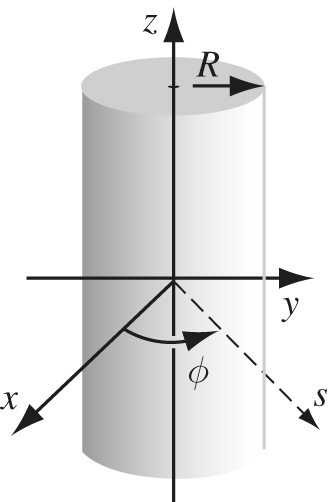
\includegraphics[width=0.15\textwidth]{figures/6_13.jpg}
\caption{\label{fig:1} A cylinder with $\mathbf{M} = ks^2\hat{\mathbf{z}}$.}
\end{figure}

\section{Memory Bank}

\begin{itemize}
\item \textbf{Bound volume current density}:
\begin{equation}
\mathbf{J}_{\rm b} = \nabla \times \mathbf{M}
\end{equation}
\item \textbf{Bound surface current density}:
\begin{equation}
\mathbf{K}_{\rm b} = \mathbf{M} \times \hat{\mathbf{n}}
\end{equation}
\item \textbf{Auxiliary field, $\mathbf{H}$}:
\begin{equation}
\mathbf{H} = \frac{1}{\mu_0}\mathbf{B}-\mathbf{M}
\end{equation}
\item \textbf{Amp\`{e}re's Law}, integral form:
\begin{equation}
\oint \mathbf{B} \cdot d\mathbf{l} = \mu_0 I_{\rm enc}
\end{equation}
\item \textbf{Amp\`{e}re's Law}, differential form:
\begin{equation}
\nabla \times \mathbf{B} = \mu_0 \mathbf{J}
\end{equation}
\end{itemize}

\vspace{1cm}

\section{Fields of Magnetized Objects}

\begin{enumerate}
\item A very long circular cylinder of radius $R$ carries a magnetization $\mathbf{M} = ks^2\hat{\boldsymbol{\phi}}$, where $k$ is a constant (Fig. \ref{fig:1}).  Find the magnetic field due to $\mathbf{M}$, for points inside and outside the cylinder. \textit{Hint: what is the total current due to bound surface and volume current densities?}\\ \vspace{4cm}
\item In the previous exercise, what is the auxiliary field, $\mathbf{H}$? \\ \vspace{2cm}
\end{enumerate}

\section{The Auxiliary Field, $\mathbf{H}$}

\begin{enumerate}
\item (a) Break the current density in Amp\`{e}re's Law (differential form) into \textit{bound} and \textit{free} current densities.  (b) Substitute the bound current density with its definition in terms of magnetization.  (c) Gather the curls on one side of the formula to find Amp\`{e}re's Law in matter.  (d) Produce the integral form. \\ \vspace{2.5cm}
\item What is the \textit{divergence} of $\mathbf{H}$? \\ \vspace{1cm}
\item An infinitely long cylinder of radius $R$ carries a magnetization $\mathbf{M} = ks \hat{\mathbf{z}}$, where $k$ is a constant, $s$ is the distance from the axis, and $\mathbf{J}_{\rm f}=0$. (a) Locate the bound currents and calculate the fields. (b) Use Amp\`{e}re's Law to find $\mathbf{H}$, and then obtain $\mathbf{B}$.
\end{enumerate}

\end{document}
